\chapter{Opis projektnog zadatka}
		
		%\textbf{\textit{dio 1. revizije}}\\
		
%		\textit{Na osnovi projektnog zadatka detaljno opisati korisničke zahtjeve. Što jasnije opisati cilj projektnog zadatka, razraditi problematiku zadatka, dodati nove aspekte problema i potencijalnih rješenja. Očekuje se minimalno 3, a poželjno 4-5 stranica opisa.	Teme koje treba dodatno razraditi u ovom poglavlju su:}
%		\begin{packed_item}
%			\item \textit{potencijalna korist ovog projekta}
%			\item \textit{postojeća slična rješenja (istražiti i ukratko opisati razlike u odnosu na zadani zadatak). Dodajte slike koja predočavaju slična rješenja.}
%			\item \textit{skup korisnika koji bi mogao biti zainteresiran za ostvareno rješenje.}
%			\item \textit{mogućnost prilagodbe rješenja }
%			\item \textit{opseg projektnog zadatka}
%			\item \textit{moguće nadogradnje projektnog zadatka}
%		\end{packed_item}
		
%		\textit{Za pomoć pogledati reference navedene u poglavlju „Popis literature“, a po potrebi konzultirati sadržaj na internetu koji nudi dobre smjernice u tom pogledu.}
		\textit{Cilj projekta je izgraditi web-aplikaciju koja će omogućiti korisnicima praćenje cijena proizvoda u trgovinama u kojoj cijene ažuriraju registrirani korisnici uz prikladne nagrade za aktivnost. Zamislimo sljedeću situaciju: Mario, student Fakulteta elektrotehnike i računarstva, želi minimizirati potrošnju novca na svakodnevne namirnice koje nabavlja u obližnjim trgovinama. Kako bi to učinio, Mario prati kataloge koje pronađe na web-stranicama istih trgovina te nakon pronalaska (ili ne pronalaska) određenih proizvoda razmisli isplati li mu se otići u najbližu trgovinu ili je bolje posjetiti više njih. Ovdje se javljaju očiti problemi da nije sve na jednom mjestu te nerijetko ti katalozi uopće nisu pretraživi. Drugi će se korisnici možda odlučiti na fizičke kataloge koji su loša opcija i za okoliš i za pretraživanje. Još jedna mana kataloga jest da ne prikazuju cijene svih proizvoda, nego samo onih sniženih.}\\
		
		\textit{Kao rješenje na navedene probleme nastaje aplikacija CjenikSvega. Svi proizvodi s cijenama u stvarnom vremenu na jednom mjestu. Aplikacija će biti od najveće koristi osobi koja živi u blizini nekoliko različitih trgovina, na primjer student u domu ili odrasla osoba u gradskoj četvrti.}\\
		
		\textit{Ta osoba kao \textbf{neregistrirani} korisnik može pregledavati i pretraživati sadržaj aplikacije. Odluči li se \textbf{registrirati}, dodatno će moći unositi cijene proizvoda i dodavati oznake (engl. tag) proizvodima. Pri registraciji osoba unosi svoje ime, prezime, nadimak i e-mail adresu. Korisnik svoje podatke može uređivati, može odabrati što će od podataka biti javno te može obrisati korisnički račun. Korisniku je u interesu registrirati se zbog nagrađivanja aktivnih korisnika i zbog mogućnosti personaliziranog popisa proizvoda koji se automatski ažurira. Jedan od primjera korištenja aplikacije jest da registrirani korisnik opazi razliku u cijenama proizvoda u trgovini i na aplikaciji te uslika taj proizvod s cijenom. Sliku će preko sučelja postaviti na web odakle će administrator odobriti izmjenu cijene. Dogodi li se da je to već treća ili neka druga proizvoljna izmjena cijene, trgovina će nagraditi korisnika s npr. 10\% popusta pri idućoj kupnji. Valja napomenuti da korisnik šalje sliku jedino kada postoji odstupanje u cijeni. Ako administrator potvrdi promjenu cijene, šalje se obavijest i korisniku i trgovini. Pohranjuju se sve promjene koje su nastale intervencijom korisnika te se to bilježi na stranici trgovine kao krivi unos.}\\
		
		\textit{\textbf{Administrator} ima sve mogućnosti kao i registrirani korisnik. Uz to može zabraniti pristup stranici registriranim korisnicima ili trgovinama i napisati komentar o svakoj pojedinoj trgovini koji je onda istaknut na stranicama trgovine. Dakle, 
pronađu li se neki korisnici koji pokušaju prevariti sistem lažiranim fotografijama proizvoda i cijena, administrator će ih blokirati i zabraniti pristup aplikaciji. Primjer jednog komentara kojeg bi administrator mogao ostaviti trgovini jest: "Trgovina xy u posljednjih mjesec dana nije imala nijedan pogrešan unos cijena."}\\
		
		\textit{\textbf{Trgovine} se registriraju na aplikaciju kako bi postavljale cijene \textbf{vlastitih} proizvoda. Prilikom registracije trgovina mora unijeti popis svih svojih proizvoda i njihove standardne cijene. Trgovina svaki dan ažurira cijene koje odstupaju od standardnih tako što postavi datoteku na računalo koju aplikacija automatski dohvaća. U slučaju da nema promjena, aplikacija pretpostavlja da za taj dan vrijede sve standardne cijene. [Trgovine mogu ponuditi kupone s popustom za aktivne korisnike koji su ispravili određen broj cijena kako bi potaknule aktivnost korisnika, a i svoje radnike u cilju smanjenja pogrešaka].}\\
		
		\textit{Svaki proizvod može imati do pet oznaka (engl. tag) vrste proizvoda. Primjeri oznaka su pekarski proizvod, mliječni proizvod, hrana, piće i slično. Konkretno za čips oznake bi mogle biti hrana, slane grickalice. Registrirani korisnici mogu predložiti do 5 oznaka po proizvodu. Prikaz oznaka određuje se većinskim glasanjem, odnosno prikazuju se onih pet za koje se najviše ljudi složilo da dobro opisuju navedeni proizvod. Svaki proizvod ima vlastitu stranicu na kojoj su prikazani detalji i slika proizvoda, sve trgovine u kojima se proizvod može kupiti te kako su se cijene mijenjale u zadnjih sedam dana u svakoj pojedinoj trgovini.}\\
		
		\textit{Rješenje problema pretraživanja jest tražilica u aplikaciji koja proizvode pretražuje po nazivu i/ili po oznakama. Osim proizvoda, mogu se pretraživati i trgovine. [Korisnik može filtrirati rezultate tražilice po cijeni, popularnosti...].}\\
		
		\textit{Rješenje koje gleda na sličan problem iz druge perspektive koje je dostupno za preuzimanje jest mobilna aplikacija Listonic, slika \ref{fig:listonic}. Glavna misao vodilja aplikacije jest da se namirnice na popisima generalno ponavljaju te umjesto da se ponovno piše popis, nudi digitalno rješenje. Razlikuje se od našeg rješenja tako što nije povezano s trgovinama koje postavljaju cijene nego korisnici sami zadaju cijene. Pogledamo li malo šire, na primjer aplikacija Basket, slika \ref{fig:basket}, mobilna aplikacija nedostupna korisnicima na ovim prostorima koja pruža uslugu dostavljanja proizvoda. Funkcionira na sličan način kao naše rješenje, trgovine postavljaju cijene koje se ažuriraju u aplikaciji te korisnici vrlo lako pronađu proizvode koji ih zanimaju. Razlike su u tome što korisnici ne ispravljaju cijene i u tome što aplikacija nudi dostavu.}\\
		
		\textit{Rješenje je moguće prilagoditi kao mobilnu aplikaciju, što bi korisnicima olakšalo samo korištenje i postavljanja fotografija. Kako bi učinili cijeli projekt profitabilnim, svakako moguća prilagodba bi bila dodati reklame i premium članstva. Provede li se prilagodba na mobilnu aplikaciju, moguće je naplaćivati samu aplikaciju nakon probnog perioda.}\\
		
		\textit{Opseg projekta je razviti web-aplikaciju s bazom podataka uz tehničku dokumentaciju. Početak je kod detaljnog definiranja zadatka u tehničkoj dokumentaciji što će dalje biti temelj projekta. Projekt se radi u dvije revizije, u prvoj reviziji isporučit će se tehnička dokumentacija sa obrascima uporabe i prikladnim dijagramima te web-aplikacija s generičkim funkcijama, dakle registracija, login i sl. U drugoj reviziji naglasak je na implementaciji te tu web-aplikacija dobija potpunu opisanu funkcionalnost. Važan dio projekta je rad i organizacija u timu od sedam članova.}\\
		
		\textit{Moguće nadogradnje su sustav za planiranje rute, dijeljenje popisa proizvoda s drugim korisnicima, dodavanje proizvoda na popis skeniranjem, prikaz proizvoda gdje se nalazi unutar trgovine. Sustav za planiranje rute bi optimizirao gdje se koji proizvod kupuje tako što uzima u obzir cijenu, udaljenost između trgovina i isplativost dodatnog putovanja. Dijeljenje popisa proizvoda s drugim korisnicima je vrlo korisno u slučaju da osoba svojoj bližnjoj osobi sastavi popis i jednostavno podijeli.}\\
		
		\begin{figure}[h]
			\begin{minipage}[t]{0.4\linewidth}
			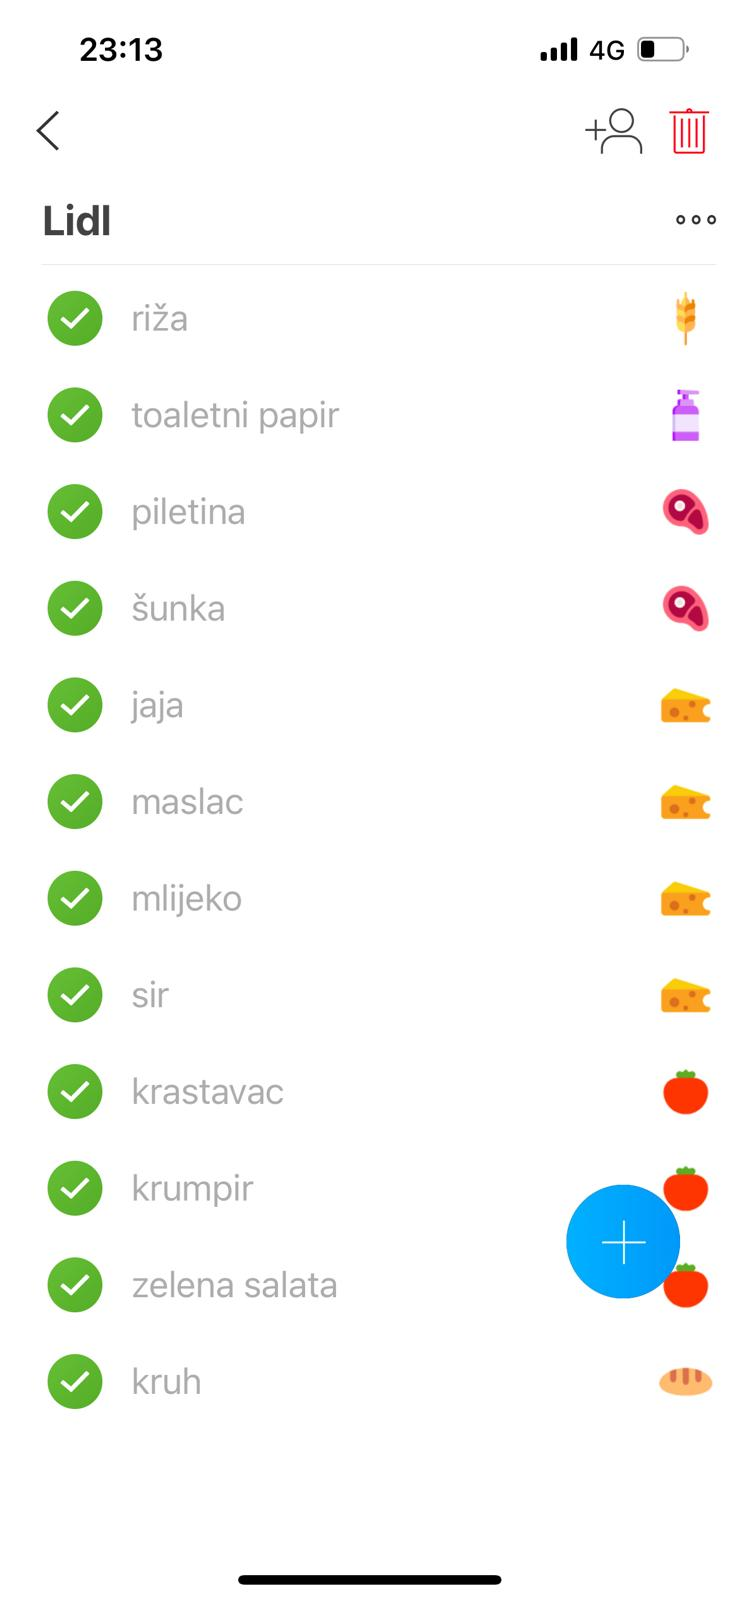
\includegraphics[width = \linewidth]{slike/listonic_primjer.JPEG}
			\centering
			\caption{Listonic}
			\label{fig:listonic}
			\end{minipage}\hfill
			\begin{minipage}[t]{0.4\linewidth}
			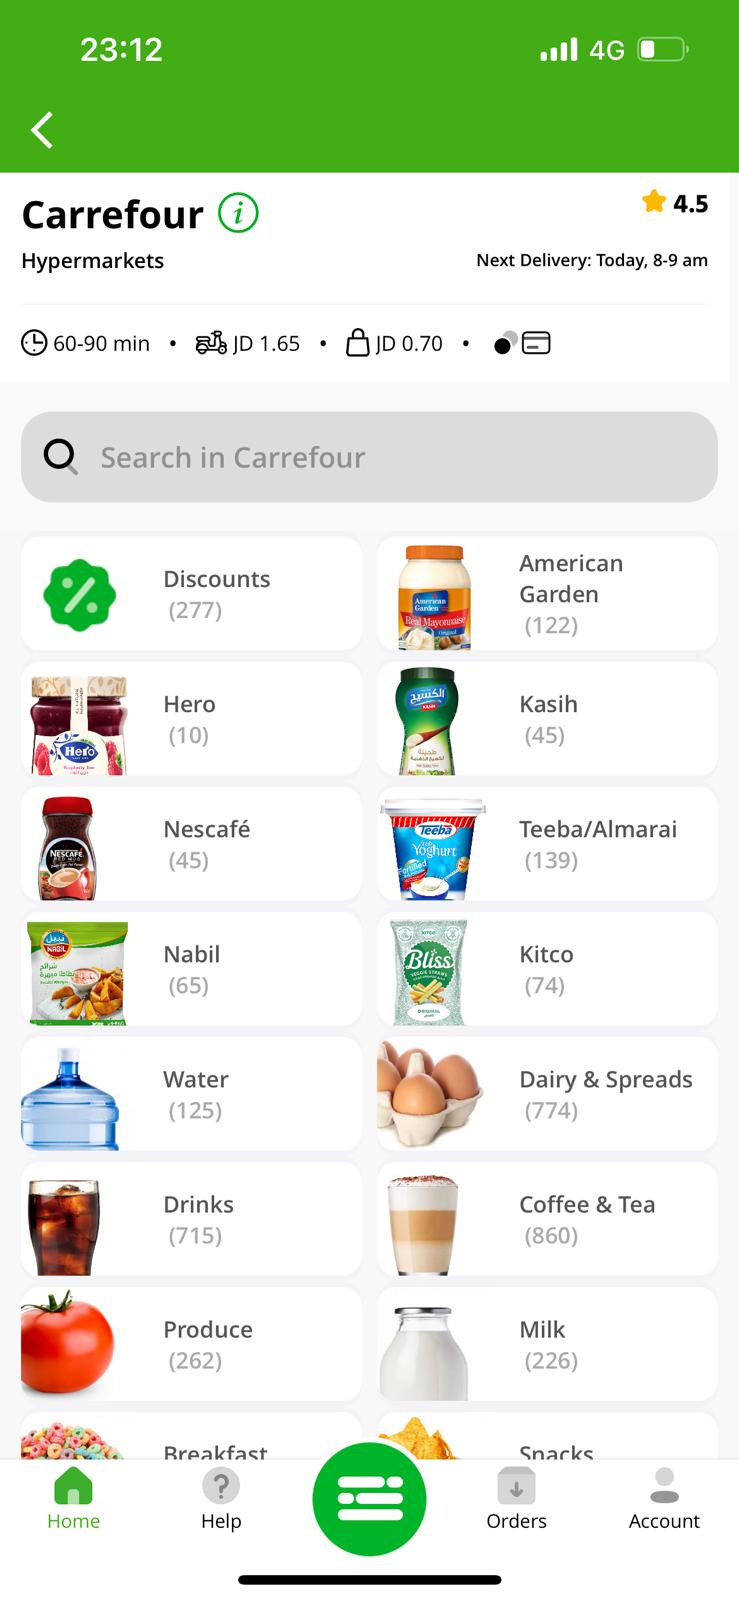
\includegraphics[width = \linewidth]{slike/basket_primjer.JPEG}
			\caption{Basket}
			\label{fig:basket}
			\end{minipage}
		\end{figure}


		\eject
		
		
		%\section{Primjeri u \LaTeX u}
		
		%\textit{Ovo potpoglavlje izbrisati.}\\

		%U nastavku se nalaze različiti primjeri kako koristiti osnovne funkcionalnosti \LaTeX a koje su potrebne za izradu dokumentacije. Za dodatnu pomoć obratiti se asistentu na projektu ili potražiti upute na sljedećim web sjedištima:
		%\begin{itemize}
		%	\item Upute za izradu diplomskog rada u \LaTeX u - \url{https://www.fer.unizg.hr/_download/repository/LaTeX-upute.pdf}
			%\item \LaTeX\ projekt - \url{https://www.latex-project.org/help/}
			%\item StackExchange za Tex - \url{https://tex.stackexchange.com/}\\
		
		%\end{itemize} 	


		
		%\noindent \underbar{podcrtani tekst}, \textbf{podebljani tekst}, 	\textit{nagnuti tekst}\\
		%\noindent \normalsize primjer \large primjer \Large primjer \LARGE {primjer} \huge {primjer} \Huge primjer \normalsize
				
		%\begin{packed_item}
			
		%	\item  primjer
		%	\item  primjer
		%	\item  primjer
		%	\item[] \begin{packed_enum}
		%		\item primjer
		%		\item[] \begin{packed_enum}
		%			\item[1.a] primjer
		%			\item[b] primjer
		%		\end{packed_enum}
		%		\item primjer
		%	\end{packed_enum}
			
		%\end{packed_item}
		
		%\noindent primjer url-a: \url{https://www.fer.unizg.hr/predmet/proinz/projekt}
		
	%	\noindent posebni znakovi: \# \$ \% \& \{ \} \_ 
	%	$|$ $<$ $>$ 
	%	\^{} 
	%	\~{} 
	%	$\backslash$ 
		
		
	%	\begin{longtblr}[
	%		label=none,
	%		entry=none
	%		]{
	%			width = \textwidth,
	%			colspec={|X[8,l]|X[8, l]|X[16, l]|}, 
	%			rowhead = 1,
	%		} %definicija širine tablice, širine stupaca, poravnanje i broja redaka naslova tablice
	%		\hline \multicolumn{3}{|c|}{\textbf{naslov unutar tablice}}	 \\ \hline[3pt]
	%		\SetCell{LightGreen}IDKorisnik & INT	&  	Lorem ipsum dolor sit amet, consectetur adipiscing elit, sed do eiusmod  	\\ \hline
	%		korisnickoIme	& VARCHAR &   	\\ \hline 
	%		email & VARCHAR &   \\ \hline 
	%		ime & VARCHAR	&  		\\ \hline 
	%		\SetCell{LightBlue} primjer	& VARCHAR &   	\\ \hline 
	%	\end{longtblr}
		

	%	\begin{longtblr}[
	%			caption = {Naslov s referencom izvan tablice},
	%			entry = {Short Caption},
	%		]{
	%			width = \textwidth, 
	%			colspec = {|X[8,l]|X[8,l]|X[16,l]|}, 
	%			rowhead = 1,
	%		}
	%		\hline
	%		\SetCell{LightGreen}IDKorisnik & INT	&  	Lorem ipsum dolor sit amet, consectetur adipiscing elit, sed do eiusmod  	\\ \hline
	%		korisnickoIme	& VARCHAR &   	\\ \hline 
	%		email & VARCHAR &   \\ \hline 
	%		ime & VARCHAR	&  		\\ \hline 
	%		\SetCell{LightBlue} primjer	& VARCHAR &   	\\ \hline 
	%	\end{longtblr}
	


		
		
		%unos slike
	%	\begin{figure}[H]
	%		\includegraphics[scale=0.4]{slike/aktivnost.PNG} %veličina slike u odnosu na originalnu datoteku i pozicija slike
	%		\centering
	%		\caption{Primjer slike s potpisom}
	%		\label{fig:promjene}
	%	\end{figure}
		
	%	\begin{figure}[H]
	%		\includegraphics[width=\textwidth]{slike/aktivnost.PNG} %veličina u odnosu na širinu linije
	%		\caption{Primjer slike s potpisom 2}
	%		\label{fig:promjene2} %label mora biti drugaciji za svaku sliku
	%	\end{figure}
		
	%	Referenciranje slike \ref{fig:promjene2} u tekstu.
		
	%	\eject
		
	
